\documentclass{chi-ext}
% Please be sure that you have the dependencies (i.e., additional LaTeX packages) to compile this example.
% See http://personales.upv.es/luileito/chiext/

\copyrightinfo{
  Permission to make digital or hard copies of all or part of this work for
  personal or classroom use is granted without fee provided that copies are
  not made or distributed for profit or commercial advantage and that
  copies bear this notice and the full citation on the first page. To copy
  otherwise, or republish, to post on servers or to redistribute to lists,
  requires prior specific permission and/or a fee.\\
  \emph{CHI'12}, May 5--10, 2012, Austin, Texas, USA.\\
  Copyright 2012 ACM 978-1-4503-1016-1/12/05...\$10.00.\\
}

\title{SIGCHI Extended Abstracts Sample File: Note Initial Caps}

\numberofauthors{8}
% Notice how author names are alternately typesetted to appear ordered in 2-column format;
% i.e., the first 4 autors on the first column and the other 4 auhors on the second column.
% Actually, it's up to you to strictly adhere to this author notation.
\author{
  \vspace{4em} % lisatolles: The abstract heading should start at the time height on the page as the authors names
  \alignauthor{
  	\textbf{First Author}\\
  	\affaddr{AuthorCo, Inc.}\\
  	\affaddr{123 Author Ave.}\\
  	\affaddr{Authortown, PA 54321 USA}\\
  	\email{author1@anotherco.com}
  }\alignauthor{
  	\textbf{Fourth Author}\\
  	\affaddr{AuthorCo, Inc.}\\
  	\affaddr{123 Author Ave.}\\
  	\affaddr{Authortown, PA 54321 USA}\\
  	\email{author4@anotherco.com}
  }\vfil
  \alignauthor{
  	\textbf{Second Author}\\
  	\affaddr{AuthorCo, Inc.}\\
  	\affaddr{123 Author Ave.}\\
  	\affaddr{Authortown, PA 54321 USA}\\
  	\email{author2@anotherco.com}
  }\alignauthor{
  	\textbf{Fifth Author}\\
  	\affaddr{AuthorCo, Inc.}\\
  	\affaddr{123 Author Ave.}\\
  	\affaddr{Authortown, PA 54321 USA}\\
  	\email{author5@anotherco.com}
  }\vfil
  \alignauthor{
  	\textbf{Third Author}\\
  	\affaddr{AuthorCo, Inc.}\\
  	\affaddr{123 Author Ave.}\\
  	\affaddr{Authortown, PA 54321 USA}\\
  	\email{author3@anotherco.com}
  }\alignauthor{
  	\textbf{Sixth Author}\\
  	\affaddr{AuthorCo, Inc.}\\
  	\affaddr{123 Author Ave.}\\
  	\affaddr{Authortown, PA 54321 USA}\\
  	\email{author6@anotherco.com}
  }
}

% Paper metadata (use plain text, for PDF inclusion and later re-using, if desired)
\def\plaintitle{SIGCHI LaTeX Extended Abstracts Template}
\def\plainauthor{Luis A. Leiva}
\def\plainkeywords{Guides, instructions, author's kit, conference publications}
\def\plaingeneralterms{Documentation, Standardization}

\hypersetup{
  % Your metadata go here
  pdftitle={\plaintitle},
  pdfauthor={\plainauthor},  
  pdfkeywords={\plainkeywords},
  pdfsubject={\plaingeneralterms},
  % Quick access to color overriding:
  citecolor=black,
  linkcolor=blue,
  menucolor=black,
  urlcolor=blue,
}

% Load basic packages
\usepackage{graphicx}   % for EPS use the graphics package instead
\usepackage{balance}    % useful for balancing the last columns
\usepackage{bibspacing} % save vertical space in references
\usepackage{array} 		% for vertical centering table cells


% NEW: create a shortcut to typeset table headings
\newcommand\tabhead[1]{\textbf{#1}}


\begin{document}

\maketitle

\begin{abstract}
In this sample we describe the formatting requirements for various SIGCHI related submissions 
and offer recommendations on writing for the worldwide SIGCHI readership. 
%Do not change the page size or page settings.
Please review this document even if you have submitted to SIGCHI conferences before, 
some format details have changed relative to previous years.
\end{abstract}

\keywords{Authors' choice; of terms; separated; by semi-colons}
\textcolor{red}{Mandatory section to be included in your final version.}

\category{H.5.m}{Information interfaces and presentation (e.g., HCI)}{Miscellaneous}. 
See: \url{http://www.acm.org/about/class/1998/} 
\textcolor{red}{Mandatory section to be included in your final version.}

\terms{}
See list of the limited ACM 16 terms in the instructions and additional information:\\
\url{http://sheridanprinting.com/sigchi/generalterms.htm}\\
\textcolor{red}{Optional section to be included in your final version.}

% =============================================================================
\section{Introduction}
% =============================================================================
This format is to be used for submissions that are published in the conference publications. 
We wish to give this volume a consistent, high-quality appearance.
We therefore ask that authors follow some simple guidelines.
In essence, you should format your paper exactly like this document. 
The easiest way to do this is simply to download a template from the conference website and replace the content with your own material.

% =============================================================================
\section{ACM Copyrights \& Permission Policy}
% =============================================================================
Accepted extended abstracts and papers will be
distributed in the Conference Publications. They will
also be placed in the ACM Digital Library, where they
will remain accessible to thousands of researchers and
practitioners worldwide. To view ACM’s copyright and
permissions policy, see:
\url{http://www.acm.org/publications/policies/copyright_policy}

% =============================================================================
\section{Text formatting}
% =============================================================================
Please use an 8.5-point Verdana font, or other sans serifs font as close as possible in appearance to Verdana in which these guidelines have been set. 
(The ``Normal'' style for this document automatically gives you this font setting.)
Arial 9-point font is a reasonable substitute for Verdana as it has a similar x-height. 
Please use serif or non-proportional fonts only for special purposes, such as distinguishing source code text.

\subsection{Text styles}
% -----------------------------------------------------------------------------
This template uses the \texttt{chi-ext} \LaTeX\ class file to facilitate text formatting.
Additionally, here is an example of footnoted text.\footnote{Use footnotes sparingly, if at all.}
As stated in the footnote, footnotes should rarely be used.

\subsection{Language, style, and content}
% -----------------------------------------------------------------------------
The written and spoken language of SIGCHI is English. 
Spelling and punctuation may use any dialect of English (e.g., British, Canadian, US, etc.) provided this is done consistently. 
Hyphenation is optional. 
To ensure suitability for an international audience, please pay attention to the following:

\begin{itemize}\compresslist
\item 	
Write in a straightforward style. 
Use simple sentence structure. 
Try to avoid long sentences and complex sentence structures. 
Use semicolons carefully.
\item 	
Use common and basic vocabulary (e.g., use the word ``unusual" rather than the word ``arcane").
\item 	
Briefly define or explain all technical terms. 
The terminology common to your practice/discipline may be different in other design practices/disciplines.
\item 	
Spell out all acronyms the first time they are used in your text. 
For example, ``World Wide Web (WWW)".
\item 	
Explain local references (e.g., not everyone knows all city names in a particular country).
\item 	
Explain ``insider" comments. 
Ensure that your whole audience understands any reference whose meaning you do not describe (e.g., do not assume that everyone has used a Macintosh or a particular application).
\item 	
Explain colloquial language and puns. 
Understanding phrases like ``red herring" requires a cultural knowledge of English. 
Humor and irony are difficult to translate.
\item 	
Use unambiguous forms for culturally localized concepts, such as times, dates, currencies and numbers (e.g., ``1-5-97" or ``5/1/97" may mean 5 January or 1 May, and ``seven o'clock" may mean 7:00 am or 19:00).

\item 	
Be careful with the use of gender-specific pronouns (\emph{he, she}) and other gender-specific words (\emph{chairman, manpower, man-months}). 
Use inclusive language (e.g., \emph{she or he, they, chair, staff, staff-hours, person-years}) that is gender-neutral. 
If necessary, you may be able to use ``he" and ``she" in alternating sentences, so that the two genders occur equally often~\cite{Schwartz95}. 
\end{itemize}


\marginpar{
	\framebox{\parbox{\marginparwidth}{\flushleft
		\begin{center}\textbf{Good Utilization of this Space Sample, as Side Bar}\end{center}

		\vspace{1em}\textbf{Preparation:}
		Do not change the text box size or position.

		\vspace{1em}\textbf{Materials:}
		This can not appear higher or lower on the page 
		because of pagination and specific headers added during the indexing and pagination process. 

		\vspace{1em}\textbf{Process:} 
		A 0.75 inch rule is beneficial to break this apart from the body text. 
		The text in this text box should remain the same size as the Body Text: 
		8.5 Verdana or Arial (with use of \textbf{bold} and \textit{italics} to highlight points)

		\vspace{1em}\textbf{Images \& Figures:}
		If you have any images in color, 
		it is always good practice to print your paper out in black and white 
		to ensure that the tones and screens used in your figures reproduce well in black and white, 
		but your images will appear in full color in the electronic proceedings and in the ACM digital library. 
		Images in your document should be at least 300 or 600 dpi for quality reproduction.
	}}
}


% =============================================================================
\section{Figures}
% =============================================================================
The examples on this and following pages should help you get a feel for how screen-shots and other figures should be placed in the template. 
\emph{Be sure to make images large enough so the important details are legible and clear.}

Your document may use color figures, which are included in the page limit; the figures must be usable when printed in black and white.

You can use the \LaTeX's \texttt{marginpar} command to insert figures in the (right) margin side of the document (see \autoref{fig:marginparsample}).

\begin{figure}
  \centering
  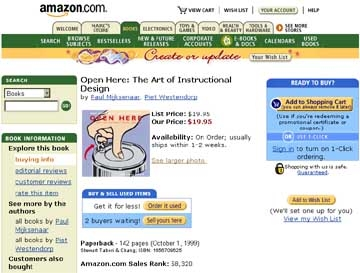
\includegraphics[width=0.7\columnwidth]{sample.jpg}
  \caption{Insert a caption below each figure.}
  \label{fig:sample}
\end{figure}

The picture format dialog has five tabs, with three---size, position, and wrapping---probably being the most useful here.

\begin{table}
\centering
	\begin{tabular}{|l|r|r|r|}
	\hline
	\tabhead{Column Head Samples} & \tabhead{1} & \tabhead{2} & \tabhead{3} \\
	\hline
	Measurements result & 22.52 & 12.16 & 10.75 \\\hline
	CogTool prediction & 22.72 & 12.26 & 10.60 \\\hline
	CogTool error \% & 0.009 & 0.008 & 0.014 \\\hline
	\end{tabular}
	\caption{This sample table has the caption appearing below.
	Please use 0.75 rules/borders for your tables, align decimals or
	center text in the cells.}\label{tab:sample}
\end{table}

As for the ``picture" tab in that dialog, we recommend using Photoshop or other graphics software to scale images.

% =============================================================================
\section{References and Citations}
% =============================================================================
Use a numbered list of references at the end of the article, ordered alphabetically by first author, and referenced by numbers in brackets \cite{Anderson92,Klemmer02,Mather00,Zellweger01}
For papers from conference proceedings, include the title of the paper and an abbreviated name of the conference (e.g., for Interact 2003 proceedings, use \emph{Proc. Interact 2003}). 
Do not include the location of the conference or the exact date; do include the page numbers if available. 
See the examples of citations at the end of this document. 

Your references should be published materials accessible to the public.  
Internal technical reports may be cited only if they are easily accessible (i.e., you provide the address for obtaining the report within your citation) and may be obtained by any reader for a nominal fee.  
Proprietary information may not be cited. 
Private communications should be acknowledged in the main text, not referenced  (e.g., [Robertson, personal communication]).



\clearpage
\marginpar{
You may want to place some marginal notes in this page to display more information.
\\[0.5\textheight]
Note that marginal notes must appear in the (left) outer margin, due to the template design.
}
\begin{figure}
\hspace*{-0.5\textwidth}% displace figure
\parbox{\textwidth}{
  \begin{center}
  \frame{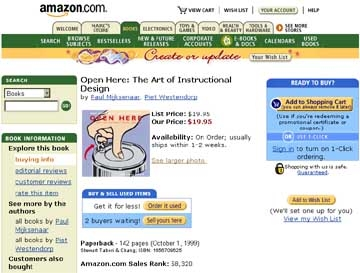
\includegraphics[width=\textwidth]{sample.jpg}}
  \caption{A big figure. You may want to place some marginal notes in this page, as shown above. Notice also that this image resolution is quite low, as it is just an example of formatting.}
  \label{fig:bigsample}
  \end{center}  
}
\end{figure}



% =============================================================================
\section{Producing and testing PDF files}
% =============================================================================
We recommend that you produce a PDF version of your submission well before the final deadline. 
\marginpar{
\begin{figure}
  \begin{center}
  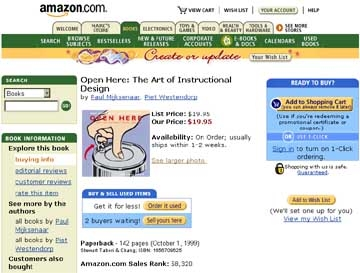
\includegraphics[width=\marginparwidth]{sample.jpg}
  \caption{A marginal figure.}
  \label{fig:marginparsample}
  \end{center}  
\end{figure}
}
Your PDF file must be ACM DL Compliant. 
The requirements for an ACM Compliant PDF are available at:
\url{http://www.sheridanprinting.com/typedept/ACM-distilling-settings.htm}

Test your PDF file by viewing or printing it with the same software we will use when we receive it, Adobe Acrobat Reader Version 7. 
This is widely available at no cost from~\cite{Acrobat7}.  
Note that most reviewers will use a North American/European version of Acrobat reader, which cannot handle documents containing non-North American or non-European fonts (e.g. Asian fonts).  
Please therefore do not use Asian fonts, and verify this by testing with a North American/European Acrobat reader (obtainable as above). Something as minor as including a space or punctuation character in a two-byte font can render a file unreadable.


% =============================================================================
\section{Dummy text}
% =============================================================================
Lorem ipsum dolor sit amet, consectetur adipiscing elit. 
\marginpar{
\begin{table}
\centering
\scriptsize
	\begin{tabular}{|c|c|c|c|}
	\hline
	\tabhead{Column} & \tabhead{1} & \tabhead{2} & \tabhead{3} \\
	\hline
	Measure & 22.52 & 12.16 & 10.75 \\\hline
	Prediction & 22.72 & 12.26 & 10.60 \\\hline
	Error \% & 0.009 & 0.008 & 0.014 \\\hline
	\end{tabular}
	\caption{This sample table has the caption appearing below.
	Please use 0.75 rules/borders for your tables, align decimals or
	center text in the cells.}\label{tab:sample}
\end{table}
}
Duis ut eros semper lectus vehicula elementum. 
Vestibulum ante ipsum primis in faucibus orci luctus et ultrices posuere cubilia Curae; 
Aliquam quis mi sapien. Suspendisse potenti. Mauris ultrices euismod velit sed dictum. Nullam auctor, nulla tincidunt dapibus suscipit, velit leo convallis metus, vel commodo libero erat in dolor. In laoreet porttitor ligula, porta blandit lectus consequat quis. 

Nam ut eros dui. Mauris volutpat elit metus, euismod pellentesque purus. In hac habitasse platea dictumst. Nullam consectetur lacinia interdum. Sed nec blandit nisi. Proin in nulla purus, sit amet iaculis tortor. Ut dapibus pellentesque nulla in interdum. Nunc at velit felis. Curabitur euismod neque eu orci varius in pharetra sem interdum. Morbi in mauris ac risus iaculis dapibus id in magna. Class aptent taciti sociosqu ad litora torquent per conubia nostra, per inceptos himenaeos.



\section{Acknowledgements}
We thank all DUX 2003 publications support and staff who wrote this document originally and allowed us to modify it for this conference.
This template was based on Manas Tungare's \texttt{chi.cls}, and rewritten by Luis A. Leiva.

\balance
\bibliographystyle{abbrv}
\bibliography{sample}

\end{document}